%package list
\documentclass{article}
\usepackage[top=3cm, bottom=3cm, outer=3cm, inner=3cm]{geometry}
\usepackage{multicol}
\usepackage{graphicx}
\usepackage{url}
%\usepackage{cite}
\usepackage{hyperref}
\usepackage{array}
%\usepackage{multicol}
\newcolumntype{x}[1]{>{\centering\arraybackslash\hspace{0pt}}p{#1}}
\usepackage{natbib}
\usepackage{pdfpages}
\usepackage{multirow}
\usepackage[normalem]{ulem}
\useunder{\uline}{\ul}{}
\usepackage{svg}
\usepackage{xcolor}
\usepackage{listings}
\lstdefinestyle{ascii-tree}{
	literate={├}{|}1 {─}{--}1 {└}{+}1 
}
\lstset{basicstyle=\ttfamily,
	showstringspaces=false,
	commentstyle=\color{red},
	keywordstyle=\color{blue}
}
%\usepackage{booktabs}
\usepackage{caption}
\usepackage{subcaption}
\usepackage{float}
\usepackage{array}

\newcolumntype{M}[1]{>{\centering\arraybackslash}m{#1}}
\newcolumntype{N}{@{}m{0pt}@{}}


%%%%%%%%%%%%%%%%%%%%%%%%%%%%%%%%%%%%%%%%%%%%%%%%%%%%%%%%%%%%%%%%%%%%%%%%%%%%
%%%%%%%%%%%%%%%%%%%%%%%%%%%%%%%%%%%%%%%%%%%%%%%%%%%%%%%%%%%%%%%%%%%%%%%%%%%%
\newcommand{\itemEmail}{jchuraaca@unsa.edu.pe}
\newcommand{\itemStudent}{Julio Rubén Chura Acabana}
\newcommand{\itemCourse}{ F. de Programción 2}
\newcommand{\itemCourseCode}{20230472}
\newcommand{\itemSemester}{I}
\newcommand{\itemUniversity}{Universidad Nacional de San Agustín de Arequipa}
\newcommand{\itemFaculty}{Facultad de Ingeniería de Producción y Servicios}
\newcommand{\itemDepartment}{Departamento Académico de Ingeniería de Sistemas e Informática}
\newcommand{\itemSchool}{Escuela Profesional de Ingeniería de Sistemas}
\newcommand{\itemAcademic}{2023 - B}
\newcommand{\itemInput}{Del 20 Septiembre 2023}
\newcommand{\itemOutput}{Al 25 Septiembre 2023}
\newcommand{\itemPracticeNumber}{03}
\newcommand{\itemTheme}{Arreglos de Objetos}
%%%%%%%%%%%%%%%%%%%%%%%%%%%%%%%%%%%%%%%%%%%%%%%%%%%%%%%%%%%%%%%%%%%%%%%%%%%%
%%%%%%%%%%%%%%%%%%%%%%%%%%%%%%%%%%%%%%%%%%%%%%%%%%%%%%%%%%%%%%%%%%%%%%%%%%%%

\usepackage[english,spanish]{babel}
\usepackage[utf8]{inputenc}
\AtBeginDocument{\selectlanguage{spanish}}
\renewcommand{\figurename}{Figura}
\renewcommand{\refname}{Referencias}
\renewcommand{\tablename}{Tabla} %esto no funciona cuando se usa babel
\AtBeginDocument{%
	\renewcommand\tablename{Tabla}
}

\usepackage{fancyhdr}
\pagestyle{fancy}
\fancyhf{}
\setlength{\headheight}{30pt}
\renewcommand{\headrulewidth}{1pt}
\renewcommand{\footrulewidth}{1pt}
\fancyhead[L]{\raisebox{-0.2\height}{
\includegraphics[width=3cm]{img/logo_episunsa.png}}}
\fancyhead[C]{\fontsize{7}{7}\selectfont	\itemUniversity \\ \itemFaculty \\ \itemDepartment \\ \itemSchool \\ \textbf{\itemCourse}}
\fancyhead[R]{\raisebox{-0.2\height}{
\includegraphics[width=1.2cm]{img/logo_abet}}}
\fancyfoot[L]{Estudiante Julio Rubén Chura Acabana}
\fancyfoot[C]{\itemCourse}
\fancyfoot[R]{Página \thepage}

% para el codigo fuente
\usepackage{listings}
\usepackage{color, colortbl}
\definecolor{dkgreen}{rgb}{0,0.6,0}
\definecolor{gray}{rgb}{0.5,0.5,0.5}
\definecolor{mauve}{rgb}{0.58,0,0.82}
\definecolor{codebackground}{rgb}{0.95, 0.95, 0.92}
\definecolor{tablebackground}{rgb}{0.8, 0, 0}

\lstset{frame=tb,
	language=bash,
	aboveskip=3mm,
	belowskip=3mm,
	showstringspaces=false,
	columns=flexible,
	basicstyle={\small\ttfamily},
	numbers=none,
	numberstyle=\tiny\color{gray},
	keywordstyle=\color{blue},
	commentstyle=\color{dkgreen},
	stringstyle=\color{mauve},
	breaklines=true,
	breakatwhitespace=true,
	tabsize=3,
	backgroundcolor= \color{codebackground},
}

\begin{document}
	
	\vspace*{10px}
	
	\begin{center}	
		\fontsize{17}{17} \textbf{ Informe de Laboratorio \itemPracticeNumber}
	\end{center}
	\centerline{\textbf{\Large Tema: \itemTheme}}
	%\vspace*{0.5cm}	
	
	\begin{flushright}
		\begin{tabular}{|M{2.5cm}|N|}
			\hline 
			\rowcolor{tablebackground}
			\color{white} \textbf{Nota}  \\
			\hline 
			\\[30pt]
			\hline 			
		\end{tabular}
	\end{flushright}	
	
	\begin{table}[H]
		\begin{tabular}{|x{4.7cm}|x{4.8cm}|x{4.8cm}|}
			\hline 
			\rowcolor{tablebackground}
			\color{white} \textbf{Estudiante} & \color{white}\textbf{Escuela}  & \color{white}\textbf{Asignatura}   \\
			\hline 
			{\itemStudent \par \itemEmail} & \itemSchool & {\itemCourse \par Semestre: \itemSemester \par Código: \itemCourseCode}     \\
			\hline 			
		\end{tabular}
	\end{table}		
	
	\begin{table}[H]
		\begin{tabular}{|x{4.7cm}|x{4.8cm}|x{4.8cm}|}
			\hline 
			\rowcolor{tablebackground}
			\color{white}\textbf{Laboratorio} & \color{white}\textbf{Tema}  & \color{white}\textbf{Duración}   \\
			\hline 
			\itemPracticeNumber & \itemTheme & 04 horas   \\
			\hline 
		\end{tabular}
	\end{table}
	
	\begin{table}[H]
		\begin{tabular}{|x{4.7cm}|x{4.8cm}|x{4.8cm}|}
			\hline 
			\rowcolor{tablebackground}
			\color{white}\textbf{Semestre académico} & \color{white}\textbf{Fecha de inicio}  & \color{white}\textbf{Fecha de entrega}   \\
			\hline 
			\itemAcademic & \itemInput &  \itemOutput  \\
			\hline 
		\end{tabular}
	\end{table}
	
	\section{Tarea}
	\begin{itemize}		
		\item 
		Debe completar el código dado en la práctica de laboratorio	
		\item Usando arreglos de objetos debe hacer la actividad 4 y 5 de la práctica 1
		\item Usted debe realizar varios commits y al término de la actividad deberá realizar un informe
	\end{itemize}
	
	\section{Equipos, materiales y temas utilizados}
	\begin{itemize}
		\item Sistema Operativo Windows
		\item VIM 9.0.
		\item OpenJDK 64-Bits 17.0.7.
		\item Git 2.39.2.
		\item Cuenta en GitHub con el correo institucional.
		\item Arreglos Estándar
	\end{itemize}
	
	\section{URL de Repositorio Github}
	\begin{itemize}
		\item URL del Repositorio GitHub para clonar o recuperar.
		\item \url{https://github.com/JulioChura/fp2-23b.git}
		\item URL para el laboratorio 01 en el Repositorio GitHub.
		\item \url{https://github.com/JulioChura/fp2-23b/tree/main/fase01/lab03}
	\end{itemize}
	
	\section{Actividades}
	
	\subsection{Completar el código de DemoBatalla.java y Nave.java}
	
	\begin{lstlisting}[language=bash,caption={Inicializando los archivos DemoBatalla.java y Nave.java}][H]
		git config --global user.name "Julio Chura"
		git config --global user.email "jchuraaca@unsa.edu.pe"
		git clone https://github.com/JulioChura/fp2-23b.git
		cd fp2-23b/fase01
		mkdir lab03
		cd lab03
		vim DemoBatalla.java
		vim Nave.java
		
		
	\end{lstlisting}
	
	\begin{lstlisting}[language=bash,caption={Commit: Subiendo archivo DemoBatalla.java incompleto }][H]
		git add DemoBatalla.java
		git add Nave.java
		git commit -m "Subiendo archivo DemoBatalla.java incompleto"
		git push
		
	\end{lstlisting}
	
		
	
	
	\begin{lstlisting}[language=bash,caption={Dándole forma y aumentando algunas líneas}][H]
		vim DemoBatalla.java	
	\end{lstlisting}
	\begin{itemize}	
		\item En el código base, se nos presenta varios métodos que debemos completar, pero nos damos cuenta que la forma en la que se imprimirá causará algo de desorden, por ello se añaden saltos de líneas y de paso se aprovecha en hacer un bosquejo del método que nos permitirá copiar los elementos de un arreglo pero de forma aleatoria.
	   \item En las líneas 28, 30, 32, 34 se añaden los saltos de línea para tener un mejor seguimiento del código al momento de imprimirse. En las líneas 35 y 36 ya se puede observar que se está implementando el método "copiarNavesAleatoriamente(Naves[] a)"
	\end{itemize}
	
	\begin{figure}[H]
		\centering
		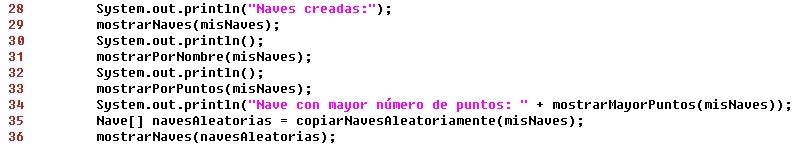
\includegraphics[width=1\textwidth,keepaspectratio]{img/1.jpg}
		%\includesvg{img/automata.svg}
		%\label{img:mot2}
		%\caption{Product backlog.}
	\end{figure}
	\begin{itemize}	
		\item En la línea 54 ya se ve la cabecera del método copiarNavesAleatoriamente(Naves[] a)
	\end{itemize}
		\begin{figure}[H]
		\centering
		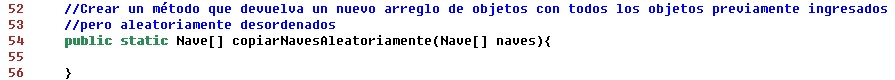
\includegraphics[width=1\textwidth,keepaspectratio]{img/2.jpg}
		%\includesvg{img/automata.svg}
		%\label{img:mot2}
		%\caption{Product backlog.}
	\end{figure}
	
	
	
	\begin{lstlisting}[language=bash,caption={Commit: Aumentando saltos de linea para una mejor presentacion y aumentando unas cosas más}][H]
		git add .
		git commit -m "Aumentando saltos  de linea para una mejor presentacion y aumentando unas cosas mas"			
		git push -u origin main
	\end{lstlisting}
	
	\begin{lstlisting}[language=bash,caption={ Completando el método mostrarNaves }][H]
		vim BatallaDemo.java
		vim Nave.java
	\end{lstlisting}
	\begin{itemize}	
		\item Para este método, se decidió recorrer todo el arreglo e ir imprimiendo, sin embargo al momento de compilar se obtuvo problemas porque en vez de imprimir los datos de cada nave, nos mostraba la dirección de memoria. 
	\end{itemize}
	\begin{figure}[H]
		\centering
		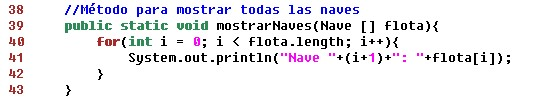
\includegraphics[width=0.8\textwidth,keepaspectratio]{img/3.jpg}
		%\includesvg{img/automata.svg}
		%\label{img:mot2}
		%\caption{Product backlog.}
	\end{figure}
	\begin{itemize}	
		\item El problema se debía a que en la clase Nave, no se escribió un método que devuelva los datos del objeto, por ello se implementa el método toString() permitiendo ahora si visualizar los datos que se han ingresado. 
	\end{itemize}
	\begin{figure}[H]
		\centering
		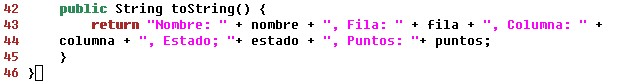
\includegraphics[width=0.9\textwidth,keepaspectratio]{img/4.jpg}
		%\includesvg{img/automata.svg}
		%\label{img:mot2}
		%\caption{Product backlog.}
	\end{figure}
	
	\begin{lstlisting}[language=bash,caption={Compilando el programa pero para ahorrar pasos, se reduce la cantidad de elementos siendo ahora de 1.}][H]
		javac Nave.java
		javac DemoBatalla.java
		java DemoBatalla
		Nave 1
		Nombre: arconte
		Fila
		3
		Columna: 4
		Estado: true
		Puntos: 34
		Naves creadas:
		Nave 1: Nombre: arconte, Fila: 3, Columna: 4, Estado; true, Puntos: 34
		Nave con mayor numero de puntos: null
	\end{lstlisting}
	
	\begin{lstlisting}[language=bash,caption={Commit:  "Metodo mostrarNaves esta terminado y modificamos el tamaño del arreglo para compilar mas rapido"}][H]
		git add .
		git commit -m "Metodo mostrarNaves esta terminado y modificamos el tamano del arreglo para compilar mas rapido""
					
		git push -u origin main
	\end{lstlisting}	
	
	\begin{lstlisting}[language=bash,caption={Completando método mostrarPorNombre }][H]
		vim DemoBatalla.java
	\end{lstlisting}

	\begin{itemize}	
		\item Para hacer la búsqueda, se decide aprovechar la propiedad que tiene el atributo Nombre de la clase Nave ya que es de tipo String, por lo que podremos usar el método equalsIgnoreCase(String str) y usaremos también el método toString() para ir imprimiendo las coincidencias. 
	\end{itemize}
	
	\begin{figure}[H]
		\centering
		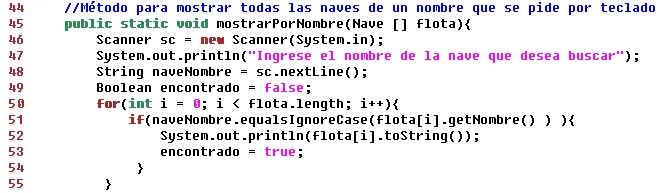
\includegraphics[width=0.9\textwidth,keepaspectratio]{img/5.jpg}
		%\includesvg{img/automata.svg}
		%\label{img:mot2}
		%\caption{Product backlog.}
	\end{figure}




	\begin{lstlisting}[language=bash,caption={Procedemos a compilar y ejecutar el programa para probar este método con una modificación en el tamaño del arreglo el cual se pondrá en 2.}][H]
		javac Nave.java
		javac DemoBatalla.java
		java DemoBatalla
		Nave 1
		Nombre: alfa
		Fila
		34
		Columna: 5
		Estado: true
		Puntos: 43
		Nave 2
		Nombre: beta
		Fila
		34
		Columna: 7
		Estado: true
		Puntos: 87
		Naves creadas:
		Nave 1: Nombre: alfa, Fila: 34, Columna: 5, Estado; true, Puntos: 43
		Nave 2: Nombre: beta, Fila: 34, Columna: 7, Estado; true, Puntos: 87
		
		Ingrese el nombre de la nave que desea buscar
		beta
		Nombre: beta, Fila: 34, Columna: 7, Estado; true, Puntos: 87
		
		Nave con mayor numero de puntos: null
	\end{lstlisting}
	

	
	\begin{lstlisting}[language=bash,caption={Commit:"Metodo para mostrar todas las naves de un nombre que se pide por teclado" }]	
		git add BatallaDemo.java
		git commit -m "Metodo para mostrar todas las naves de un nombre que se pide por teclado"
		git push -u origin main
	\end{lstlisting}
	

	
	\begin{lstlisting}[language=bash,caption={Método mostrarPorPuntos }][H]
		vim DemoBatalla.java
	\end{lstlisting}
	
	\begin{itemize}	
		\item Del mismo modo, aprovecharemos que el atributo puntos  es de tipo int para realizar un búsqueda en todo el arreglo, haremos uso de getPuntos() para ir recorriendo a lo largo del arreglo y cuando se encuentren coincidencias se imprimirán con el método toString
		\item En caso no encontrar coincidencias, se ha declarado un variable del tipo Boolean el cual se le asignó un valor de false y en caso no haber coincidencias, este boolean conservará su valor (pero si se encuentran coincidencias, su valor cambiará a true) y pasará al if ejecutándose el mensaje "No fue encontrado".
	\end{itemize}
	
	\begin{figure}[H]
		\centering
		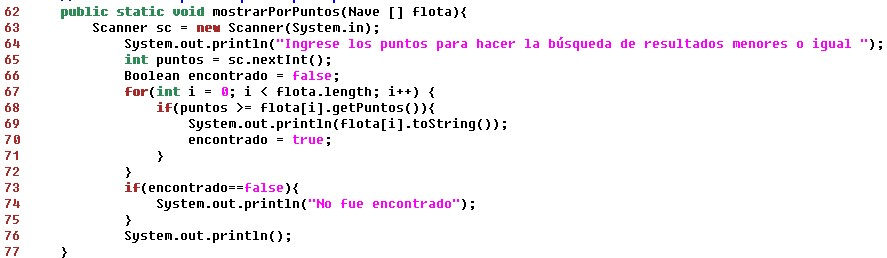
\includegraphics[width=1\textwidth,keepaspectratio]{img/6.jpg}
		%\includesvg{img/automata.svg}
		%\label{img:mot2}
		%\caption{Product backlog.}
	\end{figure}
	
	\begin{lstlisting}[language=bash,caption={Compilando y ejecutando DemoBatalla.java con este último método implemenatdo }][H]
		javac Nave.java
		javac DemoBatalla.java
		java DemoBatalla
		Nave 1
		Nombre: alfa
		Fila
		43
		Columna: 5
		Estado: true
		Puntos: 543
		Nave 2
		Nombre: beta
		Fila
		65
		Columna: 45
		Estado: true
		Puntos: 342
		Naves creadas:
		Nave 1: Nombre: alfa, Fila: 43, Columna: 5, Estado; true, Puntos: 543
		Nave 2: Nombre: beta, Fila: 65, Columna: 45, Estado; true, Puntos: 342
		
		Ingrese el nombre de la nave que desea buscar
		beta
		Nombre: beta, Fila: 65, Columna: 45, Estado; true, Puntos: 342
		
		Ingrese los puntos para hacer la busqueda de resultados menores o igual
		400
		Nombre: beta, Fila: 65, Columna: 45, Estado; true, Puntos: 342
		
		Nave con mayor numero de puntos: null
	\end{lstlisting}
	
	

	\begin{lstlisting}[language=bash,caption={Commit: Corrigiendo commit, el metodo culminado es mostrarPorPuntos }][H]
		git add .
		git commit -m "Corrigiendo commit, el metodo culminado es mostrarPorPuntos"			
		git push -u origin main
	\end{lstlisting}
	
	
	\begin{lstlisting}[language=bash,caption={Método mostrarMayorPuntos  }][H]
		vim DemoBatalla.java
	\end{lstlisting}
	
	\begin{itemize}	
		\item Del mismo modo, aprovecharemos que el atributo puntos  es de tipo int para realizar un búsqueda en todo el arreglo, haremos uso de getPuntos() para ir recorriendo a lo largo del arreglo y cuando se encuentren coincidencias se imprimirán con el método toString
		\item En caso no encontrar coincidencias, se ha declarado un variable del tipo Boolean el cual se le asignó un valor de false y en caso no haber coincidencias, este boolean conservará su valor (pero si se encuentran coincidencias, su valor cambiará a true) y pasará al if ejecutándose el mensaje "No fue encontrado"
	\end{itemize}
	
	\begin{figure}[H]
		\centering
		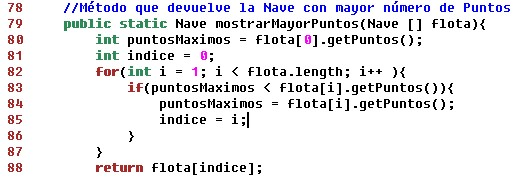
\includegraphics[width=0.8\textwidth,keepaspectratio]{img/7.jpg}
		%\includesvg{img/automata.svg}
		%\label{img:mot2}
		%\caption{Product backlog.}
	\end{figure}
	
	\begin{lstlisting}[language=bash,caption={Compilando y ejecutando el programa con 2 elementos en el arreglo  }][H]
		javac Nave.java
		javac DemoBatalla.java
		java DemoBatalla
		Nave 1
		Nombre: alfa
		Fila
		23
		Columna: 54
		Estado: true
		Puntos: 34
		Nave 2
		Nombre: beta
		Fila
		32
		Columna: 5
		Estado: true
		Puntos: 43
		Naves creadas:
		Nave 1: Nombre: alfa, Fila: 23, Columna: 54, Estado; true, Puntos: 34
		Nave 2: Nombre: beta, Fila: 32, Columna: 5, Estado; true, Puntos: 43
		
		Ingrese el nombre de la nave que desea buscar
		alfa
		Nombre: alfa, Fila: 23, Columna: 54, Estado; true, Puntos: 34
		
		Ingrese los puntos para hacer la busqueda de resultados menores o igual
		56
		Nombre: alfa, Fila: 23, Columna: 54, Estado; true, Puntos: 34
		Nombre: beta, Fila: 32, Columna: 5, Estado; true, Puntos: 43
		Nave con mayor numero de puntos: Nave 2: Nombre: beta, Fila: 32, Columna: 5, Estado; true,
	\end{lstlisting}
	
	
	\begin{lstlisting}[language=bash,caption={Commit: "Metodo mostrarMayorPuntos culmiando" }][H]
		git add .
		git commit -m  "Metodo mostrarMayorPuntos culmiando"			
		git push -u origin main
	\end{lstlisting}
	
	
	
		\begin{lstlisting}[language=bash,caption={Implementando el método copiarNavesAleatoriamente y cambiando la cantidad de elementos del arreglo, pasando de 2 a 10  }][H]
		vim DemoBatalla.java
	\end{lstlisting}
	
	\begin{itemize}	
		\item Primero se copian los elementos de un arreglo a otro, para ello se usa el método System.arrayCopy, luego se recurre a la ayuda de un algoritmo de ordenación el cual se llama Fisher-Yates shuffle que consiste en que la variable de control recorra el arreglo empezando desde la última posición, dentro del bucle se genera un número aleatorio de 0 hasta la variable de control sumado con uno, ese aleatorio representa el indice del elemento del arreglo a intercambiar con la posición en la que se encuentra la variable de control. En cada iteración la variable de control va ir disminuyendo el índice, esto con el fin de no generar números aleatorios en los espacios que ya fueron mezclados los elementos. Con el método ya realizado, lo implementamos en el main, luego cambiamos el tamaño del arreglo misNaves pasando de 2 a 10
	\end{itemize}
	
	\begin{figure}[H]
		\centering
		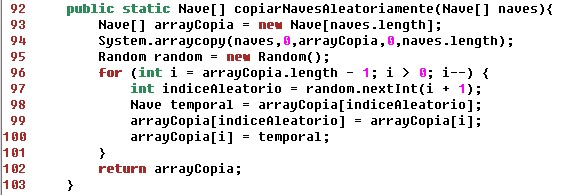
\includegraphics[width=0.8\textwidth,keepaspectratio]{img/8.jpg}
		%\includesvg{img/automata.svg}
		%\label{img:mot2}
		%\caption{Product backlog.}
	\end{figure}
	
	\begin{lstlisting}[language=bash,caption={Compilando y ejecutando el programa con 10 elementos en el arreglo  }][H]
		javac Nave.java
		javac DemoBatalla.java
		java DemoBatalla
		Nave 1
		Nombre: Alfa
		Fila
		1
		Columna: 2
		Estado: true
		Puntos: 23
		Nave 2
		Nombre: Beta
		Fila
		4
		Columna: 5
		Estado: true
		Puntos: 34
		Nave 3
		Nombre: Spider
		Fila
		6
		Columna: 4
		Estado: false
		Puntos: 56
		Nave 4
		Nombre: Caza
		Fila
		4
		Columna: 8
		Estado: true
		Puntos: 57
		Nave 5
		Nombre: Alfa
		Fila
		4
		Columna: 8
		Estado: true
		Puntos: 65
		Nave 6
		Nombre: Alcon
		Fila
		5
		Columna: 9
		Estado: true
		Puntos: 90
		Nave 7
		Nombre: Arconte
		Fila
		3
		Columna: 6
		Estado: false
		Puntos: 68
		Nave 8
		Nombre: Venganza
		Fila
		4
		Columna: 8
		Estado: true
		Puntos: 79
		Nave 9
		Nombre: Destroyer
		Fila
		4
		Columna: 7
		Estado: true
		Puntos: 34
		Nave 10
		Nombre: Huascar
		Fila
		3
		Columna: 9
		Estado: true
		Puntos: 91
		Naves creadas:
		Nave 1: Nombre: Alfa, Fila: 1, Columna: 2, Estado; true, Puntos: 23
		Nave 2: Nombre: Beta, Fila: 4, Columna: 5, Estado; true, Puntos: 34
		Nave 3: Nombre: Spider, Fila: 6, Columna: 4, Estado; false, Puntos: 56
		Nave 4: Nombre: Caza, Fila: 4, Columna: 8, Estado; true, Puntos: 57
		Nave 5: Nombre: Alfa, Fila: 4, Columna: 8, Estado; true, Puntos: 65
		Nave 6: Nombre: Alcon, Fila: 5, Columna: 9, Estado; true, Puntos: 90
		Nave 7: Nombre: Arconte, Fila: 3, Columna: 6, Estado; false, Puntos: 68
		Nave 8: Nombre: Venganza, Fila: 4, Columna: 8, Estado; true, Puntos: 79
		Nave 9: Nombre: Destroyer, Fila: 4, Columna: 7, Estado; true, Puntos: 34
		Nave 10: Nombre: Huascar, Fila: 3, Columna: 9, Estado; true, Puntos: 91
		
		Ingrese el nombre de la nave que desea buscar
		Alfa
		Nombre: Alfa, Fila: 1, Columna: 2, Estado; true, Puntos: 23
		Nombre: Alfa, Fila: 4, Columna: 8, Estado; true, Puntos: 65
		
		Ingrese los puntos para hacer la busqueda de resultados menores o igual
		70
		Nombre: Alfa, Fila: 1, Columna: 2, Estado; true, Puntos: 23
		Nombre: Beta, Fila: 4, Columna: 5, Estado; true, Puntos: 34
		Nombre: Spider, Fila: 6, Columna: 4, Estado; false, Puntos: 56
		Nombre: Caza, Fila: 4, Columna: 8, Estado; true, Puntos: 57
		Nombre: Alfa, Fila: 4, Columna: 8, Estado; true, Puntos: 65
		Nombre: Arconte, Fila: 3, Columna: 6, Estado; false, Puntos: 68
		Nombre: Destroyer, Fila: 4, Columna: 7, Estado; true, Puntos: 34
		
		Nave con mayor numero de puntos: Nombre: Huascar, Fila: 3, Columna: 9, Estado; true, Puntos: 91
		Nave 1: Nombre: Alcon, Fila: 5, Columna: 9, Estado; true, Puntos: 90
		Nave 2: Nombre: Alfa, Fila: 4, Columna: 8, Estado; true, Puntos: 65
		Nave 3: Nombre: Venganza, Fila: 4, Columna: 8, Estado; true, Puntos: 79
		Nave 4: Nombre: Destroyer, Fila: 4, Columna: 7, Estado; true, Puntos: 34
		Nave 5: Nombre: Beta, Fila: 4, Columna: 5, Estado; true, Puntos: 34
		Nave 6: Nombre: Spider, Fila: 6, Columna: 4, Estado; false, Puntos: 56
		Nave 7: Nombre: Caza, Fila: 4, Columna: 8, Estado; true, Puntos: 57
		Nave 8: Nombre: Alfa, Fila: 1, Columna: 2, Estado; true, Puntos: 23
		Nave 9: Nombre: Huascar, Fila: 3, Columna: 9, Estado; true, Puntos: 91
		Nave 10: Nombre: Arconte, Fila: 3, Columna: 6, Estado; false, Puntos: 68
		
	\end{lstlisting}
	
	
	\begin{lstlisting}[language=bash,caption={Commit: Codigo DemoBatalla.java terminado }][H]
		git add .
		git commit -m  " Codigo DemoBatalla.java terminado "			
		git push -u origin main
	\end{lstlisting}
	
	
	
	
		\subsection{Resolver la actividad 4 y 5 de la práctica01 de laboratorio pero usando arreglos de Objetos}
	
	\begin{lstlisting}[language=bash,caption={Se está copiando el archivo VideoJuego.java para resolver la actividad 4 y 5. Tambiénse está creando la clase Soldier para poder los objetos }][H]
		 cd ..
		 cd lab01
		 Copy-Item -Path "VideoJuego.java" -Destination "..\lab03"	
		 cd ..
		 cd lab03
		 vim VideoJuego.java
		 vim Soldier.java
		
	\end{lstlisting}
	
	\begin{lstlisting}[language=bash,caption={Se resuelve el ejercicio 4 de la praactica de laboratorio 01 usando arreglo con objetos.  }][H]	
	\end{lstlisting}
	
	\begin{itemize}	
		\item  Se crea la clase Soldier.java la cual contiene los atrbutos y métodos que son empleados en la clase principal. Se crea un arreglo de Soldier y para llenar dicho arreglo con los nombres y puntos de vida se usa un bucle for, en cada itereación se irá preguntando, luego se almacenarán en las variables name y lifePoint para luego mandarlos a guardar en el arreglo usando los set
	\end{itemize}
	
	\begin{figure}[H]
		\centering
		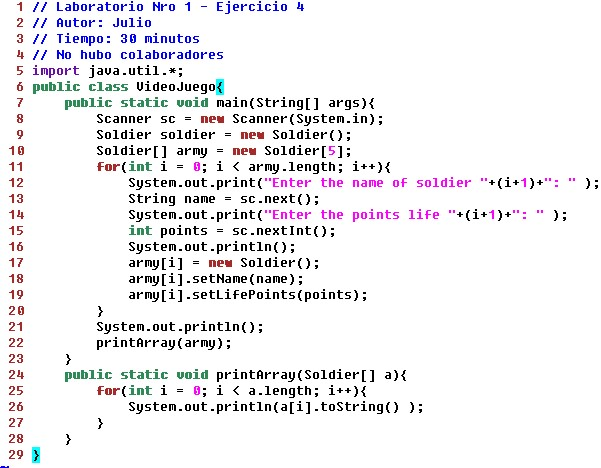
\includegraphics[width=0.8\textwidth,keepaspectratio]{img/9.jpg}
		%\includesvg{img/automata.svg}
		%\label{img:mot2}
		%\caption{Product backlog.}
	\end{figure}	
	
	\begin{lstlisting}[language=bash,caption={Commit: Se realizan 2 commit para subir tanto Soldier.java y VideoJuego.java}][H]
		git add VideoJuego.java
	    git commit -m "Ejercicio04 de lab01 usando arreglos de objetos "
	    git push -u origin main
	    git add Soldier.java
	    git commit -m "Subiendo la clase Soldier.java "	
	    gut push .u origin main
	\end{lstlisting}
	
	

	
		
	
	\begin{lstlisting}[language=bash,caption={Se realiza la actividad 5 del laboratorio01 la cual consiste en generar dos arreglos de tamaño aleatorio y gana el que tenga más soldados}][H]
		vim VideoJuego.java
	\end{lstlisting}
	
	\begin{itemize}	
		\item Se crean dos métodos, uno es para imprimir los arreglos y el otro para generar un ejército de cantidad n que está entre 1 y 5. Para determinar el ganador, se emplean condiconales donde se evalúan los tamaños de los 2 arreglos arreglos de tipo Soldier
	\end{itemize}
	
	
	\begin{figure}[H]
		\centering
		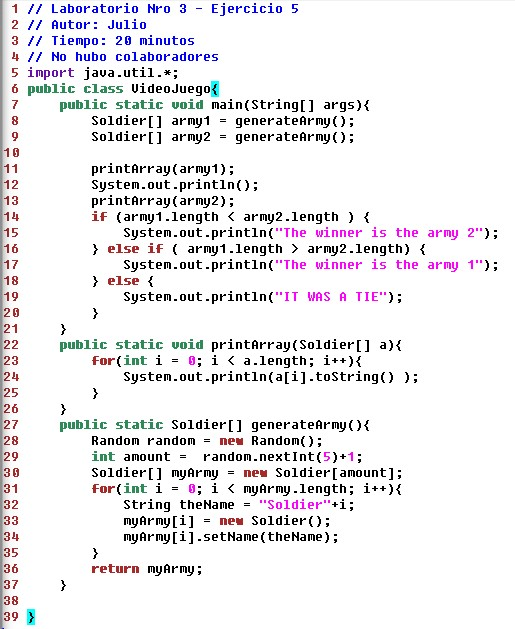
\includegraphics[width=0.7\textwidth,keepaspectratio]{img/10.jpg}
		%\includesvg{img/automata.svg}
		%\label{img:mot2}
		%\caption{Product backlog.}
	\end{figure}

	\begin{lstlisting}[language=bash,caption={Compilando y ejecutando VideoJuego.java}][H]
		javac VideoJuego.java
		javac Soldier.java
		java VideoJuego
		Soldier{name=Soldier0, lifePoints=0}
		Soldier{name=Soldier1, lifePoints=0}
		Soldier{name=Soldier2, lifePoints=0}
		
		Soldier{name=Soldier0, lifePoints=0}
		Soldier{name=Soldier1, lifePoints=0}
		Soldier{name=Soldier2, lifePoints=0}
		Soldier{name=Soldier3, lifePoints=0}
		The winner is the army 2
	\end{lstlisting}


	\begin{lstlisting}[language=bash,caption={Commit: Ejercicio 05 de la practica 01 de lab culminada }][H]
		git add VideoJuego.java
		git commit -m "Ejercicio 05 de la practica 01 de lab culminada"
		git push -u origin main
	\end{lstlisting}
	
	
	\subsection{Estructura de laboratorio 03}
	\begin{itemize}	
		\item El contenido que se entrega en este laboratorio es el siguiente:
	\end{itemize}
	
	\begin{lstlisting}[style=ascii-tree]
		lab03/
		|---DemoBatalla.java
		|---Nave.java
		|---Soldier.java
		|---VideoJuego.java
		|
		|---latex
			|---- programacion_lab03_rescobedoq_v1.0.pdf
			|-----programacion_lab03_rescobedoq_v1.0.tex
			|
			|-----img
			|       1.jpg
			|       10.jpg
			|       2.jpg
			|       3.jpg
			|       4.jpg
			|       5.jpg
			|       6.jpg
			|       7.jpg
			|       8.jpg
			|       9.jpg
			|       logo_abet.png
			|       logo_episunsa.png
			|       logo_unsa.jpg
			|
			|-----src
			
		
	\end{lstlisting}    
	
	\section{\textcolor{red}{Rúbricas}}
	
	\subsection{\textcolor{red}{Entregable Informe}}
	\begin{table}[H]
		\caption{Tipo de Informe}
		\setlength{\tabcolsep}{0.5em} % for the horizontal padding
		{\renewcommand{\arraystretch}{1.5}% for the vertical padding
			\begin{tabular}{|p{3cm}|p{12cm}|}
				\hline
				\multicolumn{2}{|c|}{\textbf{\textcolor{red}{Informe}}}  \\
				\hline 
				\textbf{\textcolor{red}{Latex}} & \textcolor{blue}{El informe está en formato PDF desde Latex,  con un formato limpio (buena presentación) y facil de leer.}   \\ 
				\hline 
				
				
			\end{tabular}
		}
	\end{table}
	
	\clearpage
	
	\subsection{\textcolor{red}{Rúbrica para el contenido del Informe y demostración}}
	\begin{itemize}			
		\item El alumno debe marcar o dejar en blanco en celdas de la columna \textbf{Checklist} si cumplio con el ítem correspondiente.
		\item Si un alumno supera la fecha de entrega,  su calificación será sobre la nota mínima aprobada, siempre y cuando cumpla con todos lo items.
		\item El alumno debe autocalificarse en la columna \textbf{Estudiante} de acuerdo a la siguiente tabla:
		
		\begin{table}[ht]
			\caption{Niveles de desempeño}
			\begin{center}
				\begin{tabular}{ccccc}
					\hline
					& \multicolumn{4}{c}{Nivel}\\
					\cline{1-5}
					\textbf{Puntos} & Insatisfactorio 25\%& En Proceso 50\% & Satisfactorio 75\% & Sobresaliente 100\%\\
					\textbf{2.0}&0.5&1.0&1.5&2.0\\
					\textbf{4.0}&1.0&2.0&3.0&4.0\\
					\hline
				\end{tabular}
			\end{center}
		\end{table}	
		
	\end{itemize}
	
	\begin{table}[H]
		\caption{Rúbrica para contenido del Informe y demostración}
		\setlength{\tabcolsep}{0.5em} % for the horizontal padding
		{\renewcommand{\arraystretch}{1.5}% for the vertical padding
			%\begin{center}
			\begin{tabular}{|p{2.7cm}|p{7cm}|x{1.3cm}|p{1.2cm}|p{1.5cm}|p{1.1cm}|}
				\hline
				\multicolumn{2}{|c|}{Contenido y demostración} & Puntos & Checklist & Estudiante & Profesor\\
				\hline
				\textbf{1. GitHub} & Hay enlace URL activo del directorio para el  laboratorio hacia su repositorio GitHub con código fuente terminado y fácil de revisar. &2 &X &2 & \\ 
				\hline
				\textbf{2. Commits} &  Hay capturas de pantalla de los commits más importantes con sus explicaciones detalladas. (El profesor puede preguntar para refrendar calificación). &4 &X &2 & \\ 
				\hline 
				\textbf{3. Código fuente} &  Hay porciones de código fuente importantes con numeración y explicaciones detalladas de sus funciones. &2 &X &2 & \\ 
				\hline 
				\textbf{4. Ejecución} & Se incluyen ejecuciones/pruebas del código fuente  explicadas gradualmente. &2 &X &2 & \\ 
				\hline			
				\textbf{5. Pregunta} & Se responde con completitud a la pregunta formulada en la tarea.  (El profesor puede preguntar para refrendar calificación).  &2 &X &2 & \\ 
				\hline	
				\textbf{6. Fechas} & Las fechas de modificación del código fuente estan dentro de los plazos de fecha de entrega establecidos. &2 &X &2 & \\ 
				\hline 
				\textbf{7. Ortografía} & El documento no muestra errores ortográficos. &2 &X &2 & \\ 
				\hline 
				\textbf{8. Madurez} & El Informe muestra de manera general una evolución de la madurez del código fuente,  explicaciones puntuales pero precisas y un acabado impecable.   (El profesor puede preguntar para refrendar calificación).  &4 &X &2 & \\ 
				\hline
				\multicolumn{2}{|c|}{\textbf{Total}} &20 & &16 & \\ 
				\hline
			\end{tabular}
			%\end{center}
			%\label{tab:multicol}
		}
	\end{table}
	
	\clearpage
	
	\section{Referencias}
	\begin{itemize}			
		\item \url{https://drive.google.com/file/d/1gF5iR4EpCOfMuwdQCGPfbErUFeA3cp_U/view?usp=drive_link}
	\end{itemize}	
	
	%\clearpage
	%\bibliographystyle{apalike}
	%\bibliographystyle{IEEEtranN}
	%\bibliography{bibliography}
	
\end{document}